\documentclass[10pt, conference, compsocconf]{IEEEtran}
\IEEEoverridecommandlockouts

% Various packages that might be useful
\usepackage[pdftex]{graphicx}
\usepackage{array}
\hyphenation{op-tical net-works semi-conduc-tor}
\usepackage{color}
\usepackage{underscore}
\usepackage{tikz}
\usepackage{algpseudocode}
\usetikzlibrary{arrows}



\begin{document}

\title{I/O Router Placement and Fine-Grained Routing on Titan to Support Spider II}

\author{\IEEEauthorblockN{Matt Ezell, Sarp Oral, Feiyi Wang, Devesh Tiwari,\\Don Maxwell, Dustin Leverman, and Jason Hill}
\IEEEauthorblockA{Oak Ridge National Laboratory; Oak Ridge, TN\\
\{ezellma,oralhs,fwang2,tiwari,maxwellde,leverman,hilljj\}@ornl.gov}
\and
\IEEEauthorblockN{David Dillow}
\IEEEauthorblockA{dave@thedillows.org}
}

\maketitle


\section{Abstract}

The Oak Ridge Leadership Computing Facility (OLCF) introduced the concept of
fine-grained routing in 2008 to improve I/O performance between the Jaguar
supercomputer and Spider, the center-wide Lustre file system. Fine-grained
routing organizes I/O paths to minimize congestion. Jaguar has since been
upgraded to Titan, providing more than a ten-fold improvement in peak
performance. To support the center’s increased computational capacity and I/O
demand, the Spider file system has been replaced with Spider II. Building on
the lessons learned from Spider, an improved method for placing LNET routers
was developed and implemented for Spider II. The fine-grained routing scripts
and configuration have been updated to provide additional optimizations and
better match the system setup. This paper presents a brief history of
fine-grained routing at OLCF, an introduction to the architectures of Titan and
Spider II, methods for placing routers in Titan, and details about the
fine-grained routing configuration.

% vim:textwidth=80:


\begin{IEEEkeywords}
Lustre; Titan; Spider II; Fine-Grained Routing; Router Placement; I/O; ORNL; OLCF
\end{IEEEkeywords}

\section{Background}

The Spider file system was designed as a center-wide shared resource to service
all Oak Ridge Leadership Computing Facility (OLCF) resources, in 2008. The
design was targeted to eliminate data islands, to reduce deployment costs, and
to increase data availability. The system was connected to Jaguar and other
OLCF resources through an InfiniBand (IB) DDR network network, named Scalable
I/O network (SION).  Each storage server was directly connected to two 108 port
IB aggregation switches.  Network translation services from Cray SeaStar to
InfiniBand was provided by Lustre Networking (LNET) routers. These routers were
also directly connected to the same two aggregation switches.    

After deployment, it was discovered that network congestion both at the Cray
SeaStar and InfiniBand networks were severely limiting aggregate I/O
performance. To solve this problem, OLCF developed and implemented a congestion
avoidance method named Fine-Grained Routing (FGR)~\cite{dillow-fgr}. FGR had
two components.  First, it paired clients to specific I/O servers that are
topologically close to each other, reducing the load on the common SeaStar
torus links and avoiding SeaStar link saturation. Second, FGR introduced a new
LNET routing configuration. This new configuration assigned varying weights to
LNET routes based on client I/O server pairings. Tests showed that with
FGR, aggregate performance was boosted by 30\%.   
 
Jaguar was upgraded to Titan in 2012. Like Jaguar, Titan has 18,688 clients.
However, each Titan node is augmented with one NVIDIA Kepler GPGPU
which increased the aggregate installed computational power by more than an
order of magnitude.  This also increased the I/O requirement. To address this
need, a new file system called Spider~II was deployed in 2013. Spider~II
provides a 4x boost in aggregate I/O performance and a 3x increase in data
storage capacity.

Spider~II was designed with a similar architecture to its predecessor,
Spider~I.  20,160 2 TB Near-Line SAS disks are organized in 8+2 RAID 6 sets
controlled by 36 DataDirect Network (DDN) SFA-12K couplets. These are
physically arranged into four rows in the data center.  The storage system is
split into two distinct, non-overlapping sections, and each is formatted as a
separate name space (atlas1 and atlas2). Each file system has 144 Lustre Object
Storage Servers (OSSs) and 1,008 Object Storage Targests (OSTs). As of
publication, a patched version of Lustre 2.4.3 is running on the I/O servers.
Each OSS is connected to one InfiniBand FDR top-of-the-rack (TOR) switch and
two DDN controllers, for reliability.  Each row has nine TOR switches (36
total).  On Titan, 440 XK7 service nodes are configured as Lustre LNET routers.
Of these, 432 are used for file I/O and 8 are for metadata communicagtion.  On
the The Titan LNET routers are directly connected to the Spider~II TOR
switches.  Table~\ref{table:component-counts} shows the quantity of each
component.

\begin{table}
 \caption{Spider~II Component Counts}
 \label{table:component-counts}
 \begin{tabular}{ | l | c | c | c | c | c | c | }
  \hline
  Count per	& Total		& FS		& Row	& SSU	& OSS	& OST	\\ \hline
  Disks		& 20,160	& 10,080	& 5,040	& 560	& 70	& 10	\\ \hline
  OSTs		& 2016		& 1008		& 504	& 56	& 7	&	\\ \hline
  OSSs		& 288		& 144		& 72	& 8	&	&	\\ \hline
  I/O Routers	& 432		& 216		& 108	& 12	&	&	\\ \hline
  IB Switches	& 36		& 18		& 9	& 1*	&	&	\\ \hline
  Rows		& 4		& 2		&	&	&	&	\\ \hline
  File Systems	& 2		&		&	&	&	&	\\ \hline
 \end{tabular}
 *Note: A given switch supports half of each of two SSUs
\end{table}

% vim:textwidth=80:

\section{Placement}

The placement of the I/O routers in a large 3D torus can have an enormous impact
on the traffic patterns and congestions characteristics present in the system.
This is important for maximizing I/O performance as well as minimizing the
interaction between application communication and I/O. Building on the lessons
learned from OLCF's Spider I implementation of fine-grained routing in 2008, an
improved method for placing LNET routers on Titan was developed and implemented
for Spider II.

\subsection{Topological Concerns}

The router placement layout used for Spider I was designed to distribute the
routers topologically through the machine while also minimizing the number of
cabinets that contained routers. This resulted in a very regular I/O pattern
that was prone to congestion if I/O traffic was not properly kept localized.

Jaguar's upgrade from Cray's SeaStar interconnect to Gemini changed the
network's characteristics.  Each Gemini supports two nodes, which effectively
halved the Y-dimension length.  Additionally, Y-dimension connections are
comprised of only half the links of X- and Z-dimension connections.  Thus, I/O
traffic should be limited in the Y-dimension due to its reduced relative
bandwidth. This suggests that routing zones should be ``flattened'' into
``rectangular prisms'' instead of the more traditional cubic zones.

Paper in \cite{interconnect}

Minimizing the hop count between clients and routers is essential for providing
high-bandwidth communications with the storage servers.  While Gemini routing
arbitration is locally fair, it is globally unfair.  Packet age and hop-count
are not taken into account when the router selects the next packet to forward.
Figure \ref{fig:geombw} shows an example of this issue.

Node 0 can be considered an I/O router while the others are acting as clients
attempting to send data to te router.  When only node 0 is communicating, it is
able to achieve 100\% of the bandwidth across the link.  Once node 2 starts
communicating, the router attached to node 1 accepts half the bandwidth from
node 1 and half from node 2.  Effectively, the bandwidth is shared between the
nodes.  When node 3 begins communicating, the router attached to node 2 fairly
arbitrates traffic between nodes 2 and 3.  Since that router only has half of
the global bandwith, nodes 2 and 3 each only get one quarter of the total
bandwith.  When node 4 begins communicating, the problem becomes even more
obvious.  The router attached to node 3 fairly arbitrates traffic between nodes
3 and 4, but it can only grant one eighth of the total bandwidth to each.


\begin{figure}[h]
  \centering
  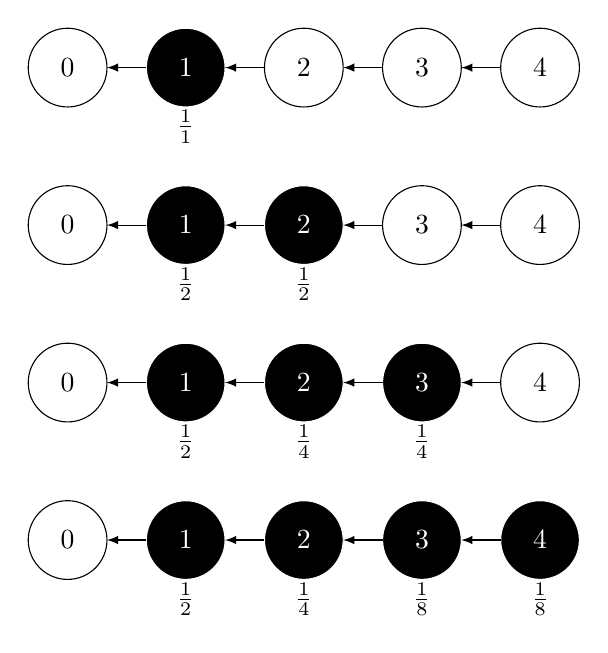
\begin{tikzpicture}
    \def \phase {1}
    \node[draw, circle, minimum height=1cm] at (0,-\phase){$0$};
    \node[draw, circle, minimum height=1cm, color=white, fill=black] at (1.5,-\phase){$1$};
    \node[draw, circle, minimum height=1cm] at (3,-\phase){$2$};
    \node[draw, circle, minimum height=1cm] at (4.5,-\phase){$3$};
    \node[draw, circle, minimum height=1cm] at (6,-\phase){$4$};
    \draw[->, >=latex] (1.0,-\phase) to (0.5,-\phase);
    \draw[->, >=latex] (2.5,-\phase) to (2.0,-\phase);
    \draw[->, >=latex] (4.0,-\phase) to (3.5,-\phase);
    \draw[->, >=latex] (5.5,-\phase) to (5.0,-\phase);
    \node[draw=none] at (1.5,-1.75) {$\frac{1}{1}$};

    \def \phase {3}
    \node[draw, circle, minimum height=1cm] at (0,-\phase){$0$};
    \node[draw, circle, minimum height=1cm, color=white, fill=black] at (1.5,-\phase){$1$};
    \node[draw, circle, minimum height=1cm, color=white, fill=black] at (3,-\phase){$2$};
    \node[draw, circle, minimum height=1cm] at (4.5,-\phase){$3$};
    \node[draw, circle, minimum height=1cm] at (6,-\phase){$4$};
    \draw[->, >=latex] (1.0,-\phase) to (0.5,-\phase);
    \draw[->, >=latex] (2.5,-\phase) to (2.0,-\phase);
    \draw[->, >=latex] (4.0,-\phase) to (3.5,-\phase);
    \draw[->, >=latex] (5.5,-\phase) to (5.0,-\phase);
    \node[draw=none] at (1.5,-3.75) {$\frac{1}{2}$};
    \node[draw=none] at (3,-3.75) {$\frac{1}{2}$};

    \def \phase {5}
    \node[draw, circle, minimum height=1cm] at (0,-\phase){$0$};
    \node[draw, circle, minimum height=1cm, color=white, fill=black] at (1.5,-\phase){$1$};
    \node[draw, circle, minimum height=1cm, color=white, fill=black] at (3,-\phase){$2$};
    \node[draw, circle, minimum height=1cm, color=white, fill=black] at (4.5,-\phase){$3$};
    \node[draw, circle, minimum height=1cm] at (6,-\phase){$4$};
    \draw[->, >=latex] (1.0,-\phase) to (0.5,-\phase);
    \draw[->, >=latex] (2.5,-\phase) to (2.0,-\phase);
    \draw[->, >=latex] (4.0,-\phase) to (3.5,-\phase);
    \draw[->, >=latex] (5.5,-\phase) to (5.0,-\phase);
    \node[draw=none] at (1.5,-5.75) {$\frac{1}{2}$};
    \node[draw=none] at (3,-5.75) {$\frac{1}{4}$};
    \node[draw=none] at (4.5,-5.75) {$\frac{1}{4}$};

    \def \phase {7}
    \node[draw, circle, minimum height=1cm] at (0,-\phase){$0$};
    \node[draw, circle, minimum height=1cm, color=white, fill=black] at (1.5,-\phase){$1$};
    \node[draw, circle, minimum height=1cm, color=white, fill=black] at (3,-\phase){$2$};
    \node[draw, circle, minimum height=1cm, color=white, fill=black] at (4.5,-\phase){$3$};
    \node[draw, circle, minimum height=1cm, color=white, fill=black] at (6,-\phase){$4$};
    \draw[->, >=latex] (1.0,-\phase) to (0.5,-\phase);
    \draw[->, >=latex] (2.5,-\phase) to (2.0,-\phase);
    \draw[->, >=latex] (4.0,-\phase) to (3.5,-\phase);
    \draw[->, >=latex] (5.5,-\phase) to (5.0,-\phase);
    \node[draw=none] at (1.5,-7.75) {$\frac{1}{2}$};
    \node[draw=none] at (3,-7.75) {$\frac{1}{4}$};
    \node[draw=none] at (4.5,-7.75) {$\frac{1}{8}$};
    \node[draw=none] at (6,-7.75) {$\frac{1}{8}$};
  \end{tikzpicture}
  \caption{Geometric Bandwidth Reductions}\label{fig:geombw}
\end{figure}

As these chains get longer and longer, the bandwidth available to the ``last''
node can become abysmal.

Minimize torus congestion

GPUs has increased load on network

Congestion avoidance

\subsection{Physical Constraints}

As part of the Spider II upgrade, the number of LNET routers on Titan was
doubled to 440 nodes and each router was equipped with an IB FDR HCA with 16
PCI-E lanes running at Gen-2.

Ensure full routability to boot from both ends

Balance router usage

Minimize Pinging

Swizzle to spread Gemini load

\subsection{Implementation}


% vim:textwidth=80:

\section{Fine-Grained Routing}

The first step towards achieving higher performance is to place LNET routers
equidistant from each other as much as possible, subject to physical
constraints and other boundary conditions. This ensures that LNET routers are
distributed across the machine and are not segregated in a particular zone. The
second key step is to pair clients with their closest possible LNET routers.
This section discusses the algorithm and implementation that pairs a client
with the optimal LNET routers to minimize hop counts and congestion.

\subsection{Router Selection Algorithm}
Recall from previous sections that there are a total of 440 LNET routers where
only 432 routers are used for file I/O; the remaining 8 are used for metadata
operations. Four LNET routers together form a router module, resulting in a
total of 108 router modules spread throughout the system. These 108 router
modules are divided into 9 groups of 12 modules each, corresponding to the 9
InfiniBand switches present in each row of Spider~II.  Each group is further
divided into 4 sub-groups that service two rows of Titan. Each sub-group
consists of 3 router modules.

Algorithm~\ref{alg:fgr} describes how a client chooses the optimal router
module for a given group. The client-to-group pairing is decided using a fixed
arrangement.  Note that in the presented algorithm $R^G_{i}(S)$ denotes
$i^{th}$ router module in the $G^{th}$ group and $S^{th}$ sub-group. Based on
the number of groups, sub-groups, and router modules in the system, $G$, $S$
and $i$ will have the following respective ranges: ($1, \dots, 9$), ($1, \dots,
4$), and ($1, \dots, 3$).

%Before we describe the algorithm in detail, we firstdescribe how 
%A router module is denoted in our algorithm depending on its association with a particular group and sub-group. The 
%$i^{th}$ router module in the $G^{th}$ group and $S^{th}$ sub-group is denoted as $R^G_{i}(S)$. 

The algorithm takes two input parameters: coordinates of the client ($C$) and
the destination router group ($R^G$). The algorithm returns the coordinates of
three routers assigned to the input client ($C$): one primary and two backup
routers. 

The fine-grained routing algorithm consists of two steps. The first step
(line~\ref{first:begin}--\ref{first:end}) is to choose the sub-group whose
Y-coordinates fall within the close range of Y-coordinates of the input client,
$C$. This is because the bandwidth in the Y-direction is limited compared to
other directions, as discussed earlier. Therefore, it is desirable to minimize
the traffic in that direction first. 

Once the sub-group is selected, the second step
(line~\ref{second:begin}--\ref{second:end}) is to return assigned routers from
this sub-group. As mentioned earlier, each sub-group consists of 3 routers and
the algorithm returns a vector of 3 routers. So, all three of them are
returned, but the one with the lowest distance in X-dimension is assigned as
the primary router to minimize the hops and avoid congestion in that direction.
Note that the X-direction crosses cabinet boundaries, therefore it more
desirable to minimize the hops in that direction compared to the Z-direction
that run within a cabinet in vertical direction.


\begin{algorithm}
\caption{Fine-grained routing algorithm}
\label{alg:fgr}
\begin{algorithmic}[1]
\Procedure {Route Selection Algorithm }{$R^G$, $C$} \\ 
%\hrulefill
\State Divide $R^G$ into 4 sub-groups: $R^G(1)$ \ldots $R^G(4)$.

\ForAll{sub-groups $R^G(i)$} \Comment{$i$ ranges 1 to 4}
\label{first:begin}
    \State $C[y]$ $\leftarrow$ y coordinate of $C$
    \State $R^G_{1}(i)$ $\leftarrow$ first router module in the $i^{th}$ sub-group
    \State $R^G_{1}(i)[y]$ $\leftarrow$ y coordinate of $R^G_{i}(S)$
    \If{ ($C[y] == R^G_{1}(i)[y]-1$) 
    \\ \hspace{\algorithmicindent} \hspace{\algorithmicindent}   or ($C[y] == R^G_{1}(i)[y]$)
    \\ \hspace{\algorithmicindent} \hspace{\algorithmicindent}   or ($C[y] == R^G_{1}(i)[y] + 1$) 
    \\ \hspace{\algorithmicindent} \hspace{\algorithmicindent}   or ($C[y] == R^G_{1}(i)[y] + 2$)}
    \State break with sub-group $i$ selected
    \EndIf
\EndFor
\label{first:end}

\\ 

\State $i$ $\leftarrow$ index of selected sub-group
\label{second:begin}
\State $r_1, r_2, r_3$ $\leftarrow$ first, second, and third router module 
\State \hspace{\algorithmicindent} selected sub-group $i$

\State $d_{min}$ $\leftarrow$ $\infty$ 
\State $Index_{primary}$ $\leftarrow$ $\infty$

\\

\For{$j$ in $1, \dots, 3$}
    \State $d_{current}$ $\leftarrow$ dist($C[x], r_j[x]$) \Comment{distance along $X$ dimension}
        \If{$d_{current}$ $<$ $d_{min}$}
        \State $Index_{primary}$ $\leftarrow$ $j$
        \EndIf

%    \State primary router module $\leftarrow$ min($d_min$)
%    \State backup router modules $\leftarrow$ 
%    \IndState{0} two other modules in the sub-group 
\EndFor

    \State primary router module $\leftarrow$ $R^G_{Index_{primary}}(i)$
    \State backup router modules $\leftarrow$ 
    \IndState{0} two other modules in the $i^{th}$ sub-group

    \Return $<$primary and backup router modules$>$ \\ 

\label{second:end}

\EndProcedure
\\
%\hrulefill
\end{algorithmic}
\end{algorithm}

\subsection{LNET Routing}

A quick introduction to LNET routing is helpful to understanding Titan's setup.
Lustre uses LNET for all communications between clients, routers, and servers.
Routing allows communication to span multiple network types, as long as one or
more nodes exist that can ``bridge'' the disjoint networks.  Each unique
network is given an identifying name that consists of the network type and an
arbitrary integer (for example, \textit{o2iblnd0} for the $0^{th}$ InfiniBand
network or \textit{gni101} for the $101^{st}$ Gemini network).

Each node in an LNET network has a unique Network Identifier (NID) that is in
the form \textit{identifier@network}.  The InfiniBand Lustre Networking Driver
(LND) uses the IP-over-IB address as its unique identifier
(ex.~\textit{10.10.10.101@o2iblnd0}), while the Gemini LND uses its Gemini
network ID (ex.~\textit{4044@gni101}).  It is permissible for a network
interface to have multiple NIDs assigned to it.  For example, a node with a
single InfiniBand interface may have NIDs \textit{10.10.10.101@o2ib0},
\textit{10.10.10.101@o2ib1}, and \textit{10.10.10.101@o2ib2}.  The Lustre
Manual \cite{lustre-manual} describes how to specify network settings.

In mixed-network environments, system administrators setup the LNET routing
tables on each node.  For every remote network that the node should be able to
communicate with, a list of routers should be provided.  Each router is given a
``hop count'' that indicates the relative distance between the nodes.

When a packet is ready to leave a node, the destination network ID is compared
to the list of local network IDs.  If a match is found, then the message is
sent directly to the destination.  Otherwise, the routing table must be used to
determine the next hop.  Under normal circumstances, LNET will cycle through
all the appropriate routers with the lowest hop count.  Routers with higher hop
counts will only be used if \textbf{all} routers of a lower hop count are
unavailable.  In all cases, LNET uses its source NID that matches the network
of the next hop.

\subsection{FGR in Practice}

Thirty-six IB LNET network identifiers (\textit{o2ib201} to \textit{o2ib236})
exist that correspond to the 36 IB leaf switches. Each LNET router has exactly
one IB NI that corresponds to the switch to which it connects.  The service and
compute nodes are broken up into twelve Gemini regions (\textit{gni101} to
\textit{gni112}) based on their topological location.  Each router configures 3
\textit{gni} interfaces corresponding to the three indices in the topological
section.

Upon boot, each client applies Algorithm~\ref{alg:fgr} for all groups A to I.
The node will create a \textit{gni} interface corresponding to each primary
router.  The primary router is added to the routing table with hop count 1
while the secondaries are added with hop count 10.  In the end, each client
will have 36 primary routes (one for each IB switch) and 72 secondary routes.

Additionally, \textit{gni100} is configured on all clients for metadata and
Cray DVS traffic.  Lustre metadata traffic uses all 8 metadata routers; it does
not use fine-grained routing.

The Lustre servers each configure one \textit{o2iblnd} network identifier that
corresponds to its IB leaf switch.  Routes for all 12 \textit{gni} networks are
configured through the 12 routers also connected to the same switch.

% vim:textwidth=80:

% vim:textwidth=80:
\section{Issues and Future Work}

- Differences depending on placement

The I/O router placement attempts to address the issue of traffic routing and
imbalance at the system level. The route selection algorithm aims to minimize
hops and mitigate contention between the compute clients and I/O routers.
However, several issues remain.

Titan's scheduler is completely oblivious to the placement of I/O routers; jobs
are placed based on node availability.  No mechanism exists for nodes to
request locality to or distance from I/O routers.  A job placed entirely within
one section (two rows) of the machine, for example, will never be able to
achieve greater than $\frac{1}{4}$ of the total file system bandwidth.
Identical jobs placed in different sections of the machine may have widely
varying locality to routers.  To users, this manifests as I/O variability.

Benchmark tests against Spider~II have been run using both optimally placed and
randomly placed clients.  On a quiet system the difference between the two
modes is minimal.  However, on a busy system the difference can be more
substantial.  Arbitrary users jobs have no insight into which ranks are closest
to I/O routers.  To overcome this limitation, OLCF is designing an end-to-end
balanced data placement strategy to complement the backend fine grained routing
algorithm. The primary goal is to extend the balancing from the clients,
through the I/O routers, and into the final destination. This work is ongoing.

While the concepts and algorithms behind fine-grained routing are
straightforward, the actual implementation is quite complex.  When issues
arise, it can be difficult narrow down to find the root cause.  Over time,
various scripts have been developed to ensure all nodes are cabled correctly
and that they can communicate properly.  Additional work improving these
scripts will aid in timely debugging.

\section{Conclusion}

The evolution of compute platforms at Oak Ridge National Laboratory has
necessitated unique designs for the storage systems that support them.  Lessons
learned from the deployment and operation of the Spider~I file system led to
the development of fine-grained routing to improve throughput and minimize
congestion.  The Spider~II system was designed and built with fine-grained
routing as a core component.  To support this new file system, the quantity of
I/O routers in Titan was increased and they were carefully placed to minimize
congestion.  A new fine-grained routing mechanism was created that was tailored
specifically to the two systems.

% vim:textwidth=80:

\section{Acknowledgement}

This research used resources of the Oak Ridge Leadership Computing Facility,
located in the National Center for Computational Sciences at Oak Ridge National
Laboratory, which is supported by the Office of Science of the Department of
Energy under Contract DE-AC05-00OR22725.

Notice: This manuscript has been authored by UT-Battelle, LLC, under Contract
No. DE-AC05-00OR22725 with the U.S. Department of Energy. The United States
Government retains and the publisher, by accepting the article for publication,
acknowledges that the United States Government retains a non-exclusive,
paid-up, irrevocable, world-wide license to publish or reproduce the published
form of this manuscript, or allow others to do so, for United States Government
purposes.

% vim:textwidth=80:



% references section
\bibliographystyle{IEEEtran}
\bibliography{cug14-fgr}
%\bibliography{IEEEabrv,cug14-fgr}

% that's all folks
\end{document}


